% \documentclass[10pt]{scrartcl}
\documentclass[10pt,twocolumn]{scrartcl}

\usepackage[utf8]{inputenc}
\usepackage[T1]{fontenc}
\usepackage[ngerman]{babel}

\usepackage{amsmath}
\usepackage{amssymb}

\usepackage{graphicx}
\usepackage{tabularx}
\usepackage{authoraftertitle}

\setlength{\parindent}{0cm}
\setlength{\parskip}{3mm}
\setlength{\textheight}{23.8cm}
\setlength{\headheight}{1cm}
\setlength{\topmargin}{-10mm}

\setlength{\oddsidemargin}{0cm}
\setlength{\evensidemargin}{0cm}
\setlength{\textwidth}{16cm}
\setlength{\columnsep}{8mm}

\usepackage{multicol}
\usepackage{colortbl}
\usepackage{xcolor}
\definecolor{grau}{gray}{0.95}
\definecolor{dunkelgrau}{gray}{0.85}

\usepackage[normal]{caption}
\usepackage{lipsum}

\setlength{\parindent}{5mm}
\setlength{\parskip}{0mm}

\usepackage{float}
\restylefloat{figure}

\renewcommand{\topfraction}{0.75}
\renewcommand{\textfraction}{0.2}

%###########################################################
% die Sachen mit der Kopfzeile
\usepackage{lastpage}
\usepackage{fancyhdr}
\fancyhf{} % leere alle Felder
\fancyhead[R]{\footnotesize Phillip Schichtel: phillip.dhbw@schich.tel \\ Jonas Dann: jonas.chr.dann@gmail.com}
\fancyhead[L]{\footnotesize Ausgewählte Methoden der
Datenanalyse, \\ Modellierung und Simulation - Raytracing} % Titel des Aufsatzes
\fancyfoot[C]{\footnotesize \thepage/\pageref{LastPage}}
% \fancyfoot[C]{\footnotesize \thepage}
\renewcommand{\headrulewidth}{0.4pt} % obere Trennlinie
\pagestyle{fancy}
%###########################################################

\title{Raytracing - Schattenberechnung im zweidimensionalen Raum}

\newcommand{\ownsection}[1]{\begin{center}\LARGE\bf#1\end{center}}

\begin{document}


{
  \onecolumn
  \maketitle
}

{
  \onecolumn
  \tableofcontents
}

\twocolumn[
\ownsection{\MyTitle}

\begin{center}
Phillip Schichtel (phillip.dhbw@schich.tel) \\
Jonas Dann (jonas.chr.dann@gmail.com) \\
Mannheim, Oktober 2014
\end{center}
\vspace*{5mm}
]

% \begin{multicols}{2}
\section{Abstract}
Schatten gibt es überall, wo es Licht gibt. Dies gibt es zu bedenken, wenn
Gebäude oder außernbereiche geplant werden.
Desweiteren geben Schatten flachen Objekten tiefe für das menschlische Auge.
Dies wird genutzt um in Filmen digital eingefügte Objekte realistisch aussehen zu lassen.
Im folgenden werden verschiedene Verfahren behandelt, die genutzt werden um realistische
Schatten so wohl für statische Szenen als auch für dynamische real-time Simulationen zu
berechnen.

\section{Motivation}

Architekten nutzen Licht- und Schattensimulationen um Räume zu planen,
Game-Designer nutzen Licht- und Schatten um Flachen grafiken auf dem 

Hier können Sie den Leser auf eine kleine Exkursion
vom Großen ins Kleine bis hin zu Ihrer Problemstellung mitnehmen.
Die großen Fragen, wie 'Woher kommen wir?', 'Was machen wir?' 
oder 'Und warum ist es so spannend sich mit dem zu 
beschäftigen, was Sie im folgenden lesen werden?' können Sie
hier behandeln.

Am Ende kann ein wenig zur Gliederung gesagt werden,
damit sich der Leser ein Bild vom Ganzen machen kann.

Achja, wenn man in einem Forschungsfeld unterwegs ist, dann
werden Sie womöglich ähnliche Einleitungen in verschiedenen
Artikeln finden. Böse gesagt, kennst Du eine 
Einleitung, kennst Du fast alle, was natürlich nicht
ganz wahr ist. Wenn man aber neu in einem Gebiet
ist, dann erhält man in der Einleitung einen schnellen Überblick.
Meistens finden sich die wichtigsten und aktuellsten 
Fakten und Veröffentlichungen des Forschungsgebietes in der Einleitung.

\subsection{Anwendung in Spielen}

text hier 

\subsection{Anwendung im Design}

noch mehr text hier

\subsection{Anwendung in Benutzeroberflächen}

.... noch mehr

\section{Problemstellung und Methoden}

\subsection{Umbra, Penumbra und Antumbra}

In der Theorie von Schatten wird ein Schatten in 4 Teile zerlegen.
\begin{enumerate}
 \item \emph{Umbra}, der Kernschatten, ist der Teil des Schattens der von keinerlei Licht erreicht wird.
       Wenn es nur eine Lichtquelle gibt, dann hat jeder Schatten einen Umbra.
 \item \emph{Antumbra}, der weiche Schatten, der hinter dem Umbra entsteht. Dieser Bereich entsteht nur,
       wenn die Lichtquelle größer ist, als das Objekt, dass den Schatten wirft. Der Antumbra beginnt an
       dem Punkt, an dem das Objekt die Lichtquelle nicht mehr vollständig verdecken kann und man die
       Ränder der Lichtquelle sehen kann.
 \item \emph{Penumbra}, die zwei weichen Schatten, die an den Seiten des Umbras entstehen. Diesen Bereich
       gibt es immer, wenn der Schatten nicht von einer Punktlichtquelle geworfen wird, in der realen
       Welt als immer. In diesem Bereich beginnt man die Seite der Lichtquelle zu sehen, die vorher im
       Umbra verdeckt wurde.
\end{enumerate}

Diese 3 separaten Bereiche eines Schatten sollten optisch realistisch dargestellt werden können.


\subsection{Shadow Mapping}

Schatten abbilden

\subsection{Raytracing}

Strahlen verfolgen

\subsection{Shadow Volumes}

Schatten zum Würfel

In naturwissenschaftlichen Veröffentlichungen sollte immer 
ein 'Abstract', eine 'Einleitung' und soetwas wie 'Ergebnisse und
Diskussion' vorhanden sein. Andererseits muss man sich bei den
Abschnitten wie 'Material und Methoden' und der 'Durchführung'
nicht zwingend an die Überschriften halten. 

Wichtig ist nur, dass man eingehens die Mittel, Techniken,
Methoden, vielleicht das mathematische Instrumentarium 
oder den experimentelle Aufbau erwähnt, mit welchem man 
gearbeitet hat und was essentiell zum Verständnis sein könnte.

Wenn Sie den Leser vorbereitet haben, was da kommt, dann können
Sie die große Synthese startet und ihr ganzes Setup mit allen
nötigen Parametern beschreiben, aus denen Sie letztendlich
die Ergebnisse generiert haben. Aus diesen Überlegungen heraus, 
sieht man bereits, dass die Grenzen zwischen den Bereichen 
'Material und Methoden' sowie 'Durchführung' und mitunter 
bis zu den 'Ergebnissen' verschwimmen können.

\subsection*{Ideen zum Lesen aus der Sicht eines Massenkonsumenten}

Da heutzutage enorm viele wissenschaftliche Artikel
eingereicht und veröffentlich werden, und das in zig verschiedenen
Journalen, kann niemand alles lesen und nur wenige haben die Zeit 
sehr viel zu lesen. Und da man als Leser noch andere Dinge im Leben 
vorhat, gibt es ein paar Techniken.
Diese Techniken spiegeln auch ein wenig die Bedeutung der einzelnen 
Abschnitte einer Veröffentlichung wieder.

Das Wichtigste ist natürlich die Überschrift, denn wenn diese außerhalb
der Interessensphäre des Lesers liegt, dann wird der Leser weiter suchen
und eine anderen Artikel heranziehen.

Danach wendet sich der Vielleser dem Abstract zu. Wenn dieses spannend ist,
wird dieser der Veröffentlichung mehr Zeit widmen. In Fächern wie der
Biochemie gibt es sogar Leute, die nur die Abstracts lesen, was durchaus
seine Berechtigung hat. Im diesen Abstracts stehen beispielsweise, 
wie bestimmte Proteine reagieren. Meistens ist das ausreichend für 
die eigene Forschung oder um etwas in Erfahrung zu bringen.
Übrigens sollte man im Internet theoretisch zu allen Veröffentlichung
die Abstracts mit dem Titel und den Autoren finden, die seit Anbeginn 
elektronischer Journals eingereicht wurden. Bei kostenpflichtigen 
Journals ist das Abstract wie der der Klappentext beim Buch und
entscheidet über Kauf oder Nichtkauf.

Die Diskussion könnte man als dritte Anlaufstelle nehmen. Wenn Sie 
die Ergebnisse, die im Abstract vielleicht bahnbrechend wirkten, genau 
beleuchtet wissen wollen, so sollten Sie hier mehr darüber
finden. Als Autor müßte man sich an dieser Stelle entsprechend 
kritisch mit den Ergebnissen auseinandersetzen. Auch ein Ausblick
ist manchmal sehr nett.

Als Viertes findet man noch eine hohe Informationsdichte in
Abbildungen, Diagrammen und Tabellen. Diese müssen so präsentiert werden,
dass man nicht hunderte von Zeilen Text durchforsten muss, damit man Sie versteht.
Dementsprechend braucht es eine Unterschrift bei Abbildungen und Diagrammen 
und einer Überschrift bei Tabellen wie es am Beispiel von Tab.~\ref{tab:falsch}
gezeigt wird. Achsenbeschriftungen, Einheitenangaben
und generell Übersichtlichkeit ist selbstredend zu beachten.
Andernfalls wird der Autor vielleicht als stümperhaft oder mindestens
wenig beflissentlich wahrgenommen.

\begin{table}[t]
\caption{Eine auffällig gefälschte Statistik über die Wissensaufnahme $\xi$
(in Wissenseinheit pro Minute) in Abhänigkeit von der verstrichenen Vorlesungszeit.}
\label{tab:falsch}
\centering
\begin{tabular}{cc}
\rowcolor{dunkelgrau}
Zeit [min] & $\xi$ [WE/min] \\
0 - 15 & 20 \\
\rowcolor{grau}
15 - 30 & 30 \\
30 - 45 & 42 \\
\rowcolor{grau}
45 - 60 & 70 \\
60 - 75 & 50 \\
\rowcolor{grau}
75 - 90 & 84
\end{tabular}
\end{table}

Wenn nun all das für den Leser interessant wirkte und dieser es vielleicht
selber im Detail nachvollziehen möchte, dann wird er sich wahrscheinlich
dem restlichen Text widmen.

Natürlich ist das eben Geschriebene nur eine Ideenskizze und wenn
Sie eine andere Herangehensweise an das Lesen solcher Artikel haben,
so steht dies Ihnen selbstverständlich frei.

\section{Durchführung}

\begin{figure}[H]
	\centering
	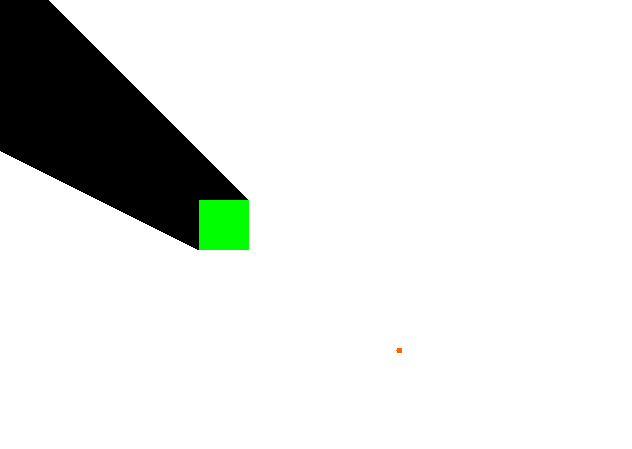
\includegraphics[width=\columnwidth]{images/durchfuehrung.png}
	\caption{Durchführung 1}
	\label{durch1}
\end{figure}

\begin{figure}[H]
	\centering
	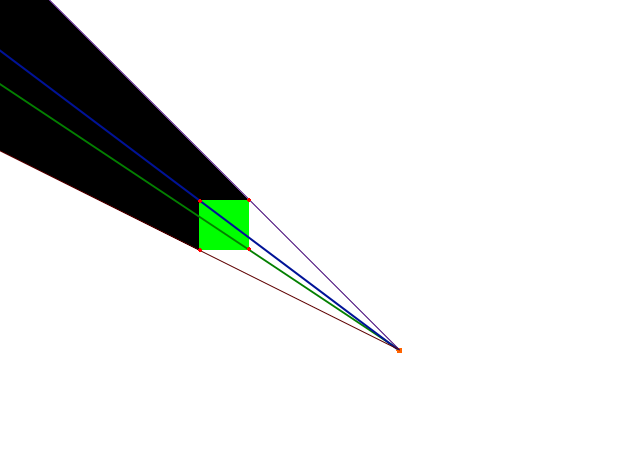
\includegraphics[width=\columnwidth]{images/durchfuehrung_1.png}
	\caption{Durchführung 2}
	\label{durch2}
\end{figure}

\begin{figure}[H]
	\centering
	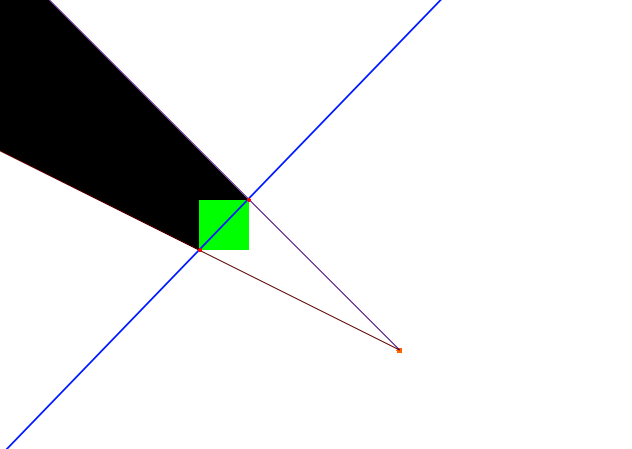
\includegraphics[width=\columnwidth]{images/durchfuehrung_2.png}
	\caption{Durchführung 3}
	\label{durch3}
\end{figure}

\begin{figure}[H]
	\centering
	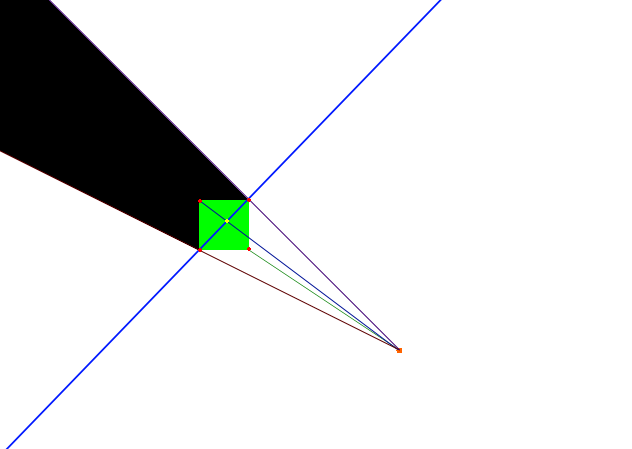
\includegraphics[width=\columnwidth]{images/durchfuehrung_3.png}
	\caption{Durchführung 4}
	\label{durch4}
\end{figure}

\begin{figure}[H]
	\centering
	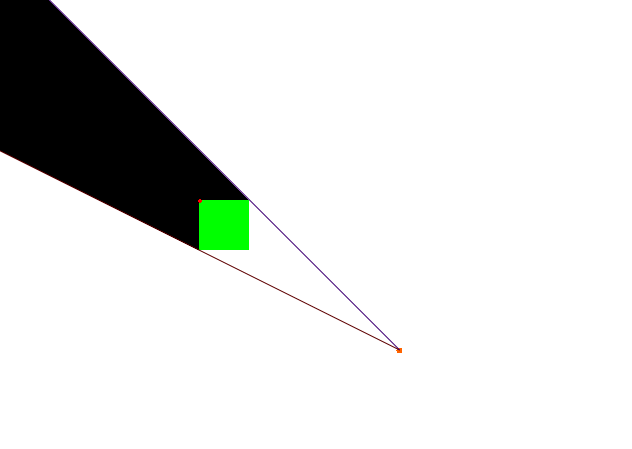
\includegraphics[width=\columnwidth]{images/durchfuehrung_4.png}
	\caption{Durchführung 5}
	\label{durch5}
\end{figure}

Hier ein paar Regeln zum Schreiben eines Artikels, 
gegen die ich teilweise in dieser Ausarbeitung bereits
verstoßen habe.
\begin{list}{-}{}
\item[(a)] Schreiben Sie nicht in 'Ich'-Form! Versuchen Sie entweder 
unpersönlich zu bleiben oder ggf. im Namen des Forschungsteams mit 'wir' zu arbeiten.

\item[(b)] Sprechen Sie den Leser nicht an! Der Leser soll sich selber ein
objektives Bild über den Artikel machen. Ich hoffe Sie verstehen das, oder?

\item[(c)] Bilder, Diagramme und Tabellen stehen alleine. Im Text findet man
nur die Referenzen darauf, wie Sie dies mit Bezug auf
Abb.~\ref{fig:audio} ersehen.

\item[(d)] Bilder, Diagramme und Tabellen sind nie vor der Seite der entsprechenden 
Referenz im Text zu finden. Meistens findet man sie gesammelt im oberen
Seitenbereich, der entsprechenden oder der nahen Folgeseiten. Die Positionierung
im oberen Bereich der Seite hilft den Schnelldurchblätterer, dass seine 
Augen nicht so viel springen müssen.

\item[(e)] Gleichungen und Formeln wie beispielsweise das Faltungsintegral
\begin{equation}
g(t) = \int_{-\infty}^{+\infty}\!\!d\tau \; h(\tau) \, f(t-\tau)
\label{eq:faltung}
\end{equation}
stehen niemals isoliert und sollen sich harmonisch in die Satzstruktur einfügen.
Es empfiehlt sich bei neuen Variablen gleich unter der Gleichung, diese
zu benennen bzw. zu erklären, damit der Leser nicht lange suchen muss.

\item[(f)] Bezieht man sich auf eine Formel, weil man beispielsweise findet,
dass die Integralschreibweise für die Korrelationsanalyse 
\begin{equation}
g(t) = \int_{-\infty}^{+\infty}\!\!d\tau \; h(\tau) \, f(t + \tau)
\end{equation}
dem Faltungsintegral aus Gl.~\eqref{eq:faltung} sehr ähnlich sieht,
so sollte man anhand der hier getätigten Referenz die Umsetzung ersehen.

\item[(g)] Zitieren Sie jemanden oder beziehen Sie sich nur auf eine
Veröffentlichung wie beispielsweise auf ein interessantes Experiment 
zur Totalreflektion \cite{Goos1947}, so können Sie dies beispielsweise 
durch Nummern tun, die im Literaturverzeichnis ausgeführt sind.
Andernorts findet man auch gern den Nachnamen des Erstautors und
das Erscheinungsjahr als Schlüssel, um den Eintrag im Literaturverzeichnis
zu finden. 

Übrigens findet man in naturwissenschaftlichen Schriften 
äußerst selten wörtliche Zitate und meist Referenzen, oder wollten Sie
aus der Arbeit von Einstein zur Speziellen Relativitätstheorie \cite{Einstein1905}
wörtlich zitieren?

\item[(h)] Das Literaturverzeichnis sollte ausreichend Informationen enthalten,
um die Veröffentlichungen auch zu finden. Ebenso muß es einheitlich für
die einzelnen Veröffentlichungstypen wie Buch, Artikel, Webseite etc. sein,
denn nur die Wenigsten mögen es, sich durch scheinbares Chaos fremder Leute zu wühlen.

\item[(i)] Argumentieren Sie! Entschuldigen Sie sich nicht für Ihre Arbeit, 
aber argumentieren und diskutieren Sie die Dinge, die merkwürdig sind.
Führen Sie weitestgehend objektive Gründe an, wenn etwas nicht funktionierte.
Argumentationen, Begründungen etc. müssen meist nicht lang sein, 
aber über offensichtliche Wiedersprüche zu schweigen wirkt unprofessionell 
und der verärgerte Leser wird vielleicht noch unliebsamere Worte 
zum Lästern finden.

\item[(j)] Vermeiden Sie Füllwörter! Obwohl man aber vielleicht auch behaupten
könnte, dass dann auch ein wenig mehr Text gefüllt wird.
\end{list}

\begin{figure}[t]
\centering
%\includegraphics[width=0.45\textwidth]{Bilder/audio-signal-short.pdf}
\caption{Das akustische Signal von etwas Gestammelten, wobei die Amplituden in 
nicht näher zu bezeichnenden Einheiten (a.u. für arbitrary unit) angegeben sind.}
\label{fig:audio}
\end{figure}

\section{Ergebnisse und Diskussion}

\begin{figure}[H]
	\centering
	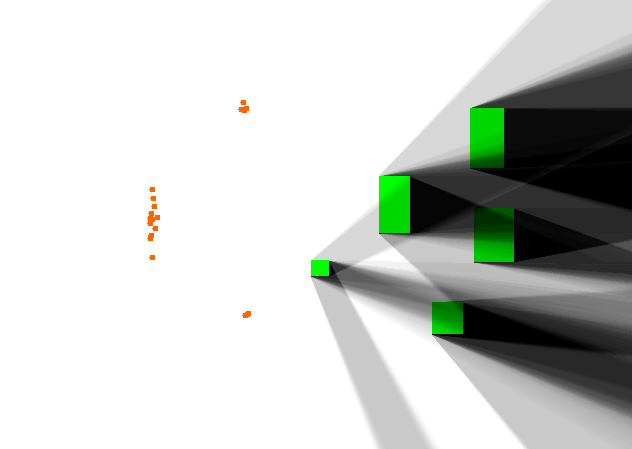
\includegraphics[width=\columnwidth]{images/ergebnis_4.png}
	\caption{Ergebnis 1}
	\label{ergeb1}
\end{figure}

\begin{figure}[H]
	\centering
	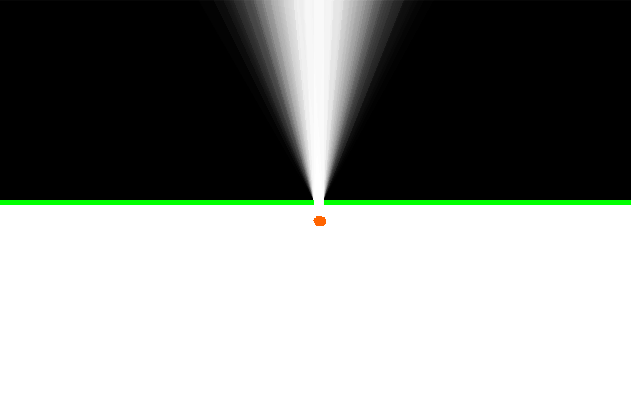
\includegraphics[width=\columnwidth]{images/ergebnis.png}
	\caption{Ergebnis 2}
	\label{ergeb2}
\end{figure}

\begin{figure}[H]
	\centering
	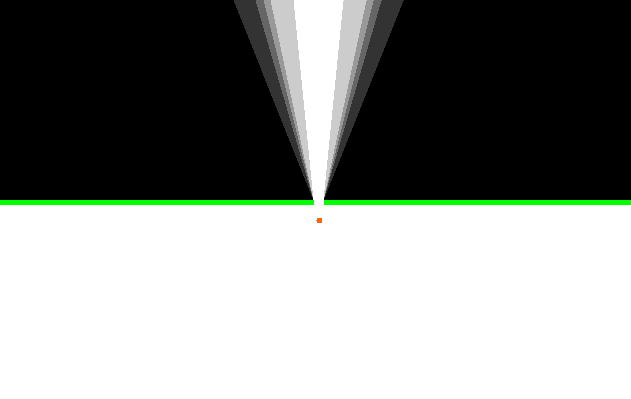
\includegraphics[width=\columnwidth]{images/ergebnis_2.png}
	\caption{Ergebnis 3}
	\label{ergeb3}
\end{figure}

\begin{figure}[H]
	\centering
	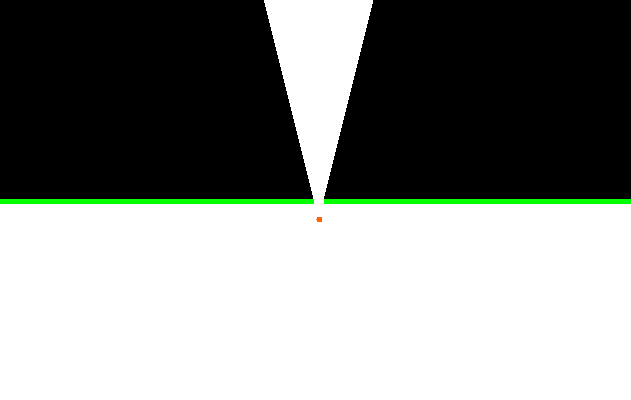
\includegraphics[width=\columnwidth]{images/ergebnis_3.png}
	\caption{Ergebnis 4}
	\label{ergeb4}
\end{figure}

Was Sie hier finden sollten, findet sich leider schon in den vorangegangenen
Textpassagen und Abschnitten und ich mag Sie nicht mit Wiederholungen
langweilen. Jedoch kann man ab und zu feststellen, dass das Abstract und
die Diskussionen eine gewisse Ähnlichkeit aufweisen, wobei die Diskussion
immer ausführlicher sein soll. Das liegt mitunter daran, dass beide 
Abschnitte Zusammenfassungen mit unterschiedlicher Nuancierung darstellen. 

Jetzt möchte ich mich gleich auf genau dieses Schreiben beziehen, 
von dem ich hoffe, dass Sie hinsichtlich des Schreibens und Lesens 
von solchen Ideen- und Gedankenmanifestationen etwas für sich mitnehmen konnten. 
Selber hatte ich mit diesem Thema verstärkt während meiner Doktorarbeit \cite{Gerhards2008} 
zu tun gehabt, ohne selber der enthusiastischste Leser gewesen zu sein.
Viele Ideen und Ansichten habe ich jedoch von meinem Doktorvater 
Prof. Dr. Kurt Roth mitbekommen, dessen arbeitsgruppeninterne Übungen 
zum schnellen Lesen förderlich für die Adrenalinproduktion waren.

% Ziel der Vorlesung war neben der sehr theorielastigen Einführung
% in die Fourier-Transformation, Faltung, Korrelationsanalyse und
% der nichtlinearen Optimierung, dass Sie sich mit einem Problem
% mit stark physikalischem Schwerpunkt auseinandersetzen sollten.
% Hier galt es sich einzuarbeiten und danach die entsprechenden
% Werkzeuge zum Lösen des Problems sowie zur graphischen Visualisierung
% anzueignen. Die Päsentation sowie der Abschlussbericht stellen
% dann die mündliche, wie schriftliche Darlegung des Problems und
% dessen Lösunng dar.
% 
% Und auch wenn Sie mit Ihrem Problem in Zukunft nie wieder in
% Berührung kommen werden, ist es generell wichtig Probleme anzugehen,
% die Werkzeuge zur dessen Bewältigung anzueignen und danach die
% Problemlösung auch voranzutreiben. Wissenschaftlichkeit in den
% Sachverhalt einfließen zu lassen, bedeutet dann noch das Problem
% in einem größeren Kontext zu sehen oder auch in Bezug auf verwandte
% Problematiken.

% Zum Abschluss aber noch einen Witz: Stellen Sie sich eine Party
% vieler mathematischer Funktionen vor. Auf einmal öffnet sich die
% Tür und ein Differentialoperator tritt herein. Alle Funktionen
% suchen die Flucht, nur die e-Funktion bleibt an der Bar stehen.
% Kommt der Differentialoperator zur e-Funktion und fragt, warum
% sie denn nicht weglaufen täte. 'Na, ich bin doch die Funktion e hoch x.
% Du kannst mich nicht wegdifferenzieren.' Darauf antwortet der
% Differentialoperator: 'Aber ich leite doch nach y ab.'

Schließen möchte ich mit einem Zitat von Wittgenstein \cite{Wittgenstein1922},
welches Prof. Dr. Kurt Roth im Zusammenhang wissenschaftlichen
Schreibens gerne nutzte: {\it Was sich überhaupt sagen lässt, lässt
sich klar sagen; und wovon man nicht reden kann, darüber muss man
schweigen.} 

\section{Diskussion}

Wenn es jemanden zu danken gibt, wie beispielsweise die Geldgeber, 
dann ist hier der Ort.

\subsection{Die Grenzen des gewählten Ansatz}

Ich für meinen Teil möchte den Dank an Prof. Dr. Tobias Straub
richten, für das Angebot eine Vorlesung an der Dualen Hochschule in
Mannheim halten zu dürfen. Auch einen Dank an all die Studenten der Vorlesung

\subsection{Alternative Ansätze}

und besonders für die spannenden Projekte, bei den ich teils auch 
etwas hinzulernen durfte. Am Ende nochmals vielen Dank 

\subsection{Abdeckung der Problematik}

an den bereits erwähnten Prof. Dr. Kurt Roth für alles, 
was ich während meiner Doktorarbeit durch ihn gelernt habe.

\begin{thebibliography}{99}
\bibitem{Goos1947}F.Goos und H.Hänchen: {\it Ein neuer fundamentaler Versuch zur Totalreflektion}, 1947; Annalen der Physik 436, S. 333-346
\bibitem{Einstein1905}A.Einstein {\it Zur Elektrodynamik bewegter Körper}, 1905; Annalen der Physik und Chemie 17, S. 891-921
\bibitem{Gerhards2008}H.Gerhards: {\it Ground Penetrating Radar as a Quantative Tool with Applications in Soil Hydrology}, Heidelberg 2008; Dissertaton,
\bibitem{Wittgenstein1922}L.Wittgenstein: {\it Tractatus Logico-Philo\-so\-phi\-cus}, London 1922; Kegan Paul, Trench, Trubner \& Co., Ltd.
\end{thebibliography}

\end{document}
